\documentclass{article}
\usepackage{amsmath}
\usepackage{hyperref}
\usepackage{tabularx}
\usepackage{tikz}
\usepackage[a4paper]{geometry}
\usepackage{fancyhdr}
\pagestyle{fancy}
\lhead{Der elektromagnetische Schwingkreis}
\rhead{März 2026}
\begin{document}
\section{Der elektromagnetische Schwingkreis}
\begin{minipage}[t]{\dimexpr\linewidth-6cm}
Wird der Schalter in Position I gelegt, so wird der Kondensator aufgeladen.
 
Wird er in Position II umgelegt, so entlädt der Kondensator sich über die Spule mit ihrem Eisenkern. Aufgrund des Stromflusses entsteht an der Spule ein magnetisches Feld. Der Selbstinduktion nach induziert dieses im der Spule weiteren Stromfluss, in die gleiche Richtung. So wird der Kondensator erneut geladen; der Zyklus ist erneut am Ausgangspunkt.
 
So schwingen sowohl das elektrische Feld des Kondensators und das Magnetfeld der Spule, jeweils Zeitversetzt.
\end{minipage}
\hfill
\begin{minipage}[t]{6cm}
 \centering
 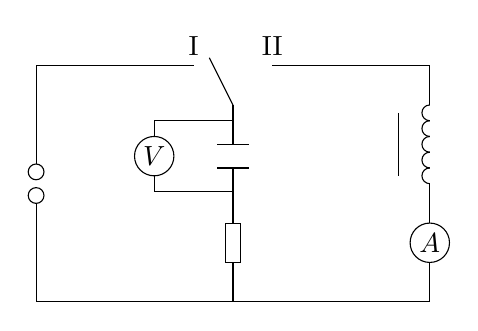
\begin{tikzpicture}[baseline=(current bounding box.north)]
  \draw (0, 0) -- (2, 0);
  \node at (2, 0) [above] {I}; 
  \draw (3, 0) -- (5, 0);
  \node at (3, 0) [above] {II}; 
  \draw (5, 0) -- (5, -0.5);  
  \begin{scope}
   \clip (3,0) rectangle (5,-2);
   \draw (5,-0.6) circle(0.1);
   \draw (5,-0.8) circle(0.1);
   \draw (5,-1.0) circle(0.1);
   \draw (5,-1.2) circle(0.1);
   \draw (5,-1.4) circle(0.1);
  \end{scope}
  \draw (4.6, -0.6) -- (4.6, -1.4); 
  \draw (5, -1.5) -- (5, -2); 
  \draw (5, -2.25) circle (0.25) node {$A$};
  \draw (5, -2.5) -- (5, -3);
  \draw (5, -3) -- (0, -3);
  \draw (2.2, 0.1) -- (2.5, -0.5);
  \draw (2.5, -0.5) -- (2.5, -1);
 
  \draw (2.3, -1) -- (2.7, -1);
  \draw (2.3, -1.3) -- (2.7, -1.3);
 
  \draw (1.5, -1.15) circle (0.25) node {$V$};
  \draw (2.5, -0.7) -- (1.5, -0.7);
  \draw (1.5, -0.9) -- (1.5, -0.7);
  \draw (2.5, -1.6) -- (1.5, -1.6);
  \draw (1.5, -1.4) -- (1.5, -1.6);
  
  \draw (2.5, -1.3) -- (2.5, -2);
  \draw (2.5, -2.5) -- (2.5, -3);
  \draw (2.4, -2) rectangle (2.6, -2.5);
 
  \draw (0, 0) -- (0, -1.25);    
  \draw (0, -1.35) circle (0.1); 
  \draw (0, -1.65) circle (0.1);
  \draw (0, -1.75) -- (0, -3);
 \end{tikzpicture}
\end{minipage} 
 
\subsection{Energieumwandlungen}
Hier schwingt die elektrischen Energie und die Energie des Magnetfeldes miteinander. Die elektrische Energie wird in in ein Magnetfeld umgewandelt; dessen Energie wird genutzt um neue elektrische Energie zu induzieren.
 
Dies steht in Analogie zu den Energieumwandlungen eines \hyperref[Das Fadenpendel]{Feder-Masse-Pendels} bei welchem die $E_\text{kin}$ und $E_\text{spann}$ einander aufbauen und zusammen schwingen.
 
\subsection{Die Resonanzkurve}
Wird in der obigen Schaltskizze der Schalter durch eine Wechselstromquelle mit einstellbarer Frequenz ersetzt und mit einem Widerstand hinter der Spule parallel ein Voltmeter geschalten, so kann die Stromquelle eine erzwungene Schwingung verursachen. Bei dieser können für unterschiedliche Werte von $f$ ein $U$ gemessen werden; diese Kurve stellt die Resonanzkurve dar.
 
Das System würde ohne der erzwungenen Schwingung eigentlich in der Eigenfrequenz schwingen. Dem Prinzip der Resonanz nach ist hier also die $U$ bei der $f_\text{eigen}$ am höchsten. So kann die Eigenfrequenz der Systems gefunden werden.
 
Wird dieser Versuch wiederholt, mit unterschiedlichen Spulen und Kondensatoren, so kann ein Zusammenhang zwischen dessen Eigenschaften und der $f_\text{eigen}$ gefunden werden.
 
\subsection{Die thomsonsche Schwingungsgleichung} 
In Abhängigkeit von der Induktivität der Spule $L$ und der Kapazität des Kondensators $C$ kann der \emph{thomsonschen Schwingungsgleichung} nach die Schwingungsdauer $T$ bestimmt werden.
\[
 T = 2\pi \cdot \sqrt{L \cdot C} 
\] 
\end{document}